%!TEX program = xelatex
\documentclass[12pt, a4paper]{article}

\usepackage[dvipsnames]{xcolor}

\usepackage{fancyhdr}
\usepackage{extramarks}
\usepackage{amsmath}
\usepackage{empheq}
\usepackage{amsthm}
\usepackage{amsfonts}
\usepackage{tikz}
\usepackage{tikz-3dplot}
\usepackage[plain]{algorithm}
\usepackage{algpseudocode}

\usepackage{ctex}
\usepackage{upgreek}
\usepackage{indentfirst}
\usepackage{wrapfig}
\usepackage{subfigure}
\usepackage{pgfplots}
\usepgfplotslibrary{patchplots}
\usepgfplotslibrary{colormaps}
\usepgfplotslibrary{colorbrewer}
\pgfplotsset{compat=1.18}
\usetikzlibrary{automata,positioning,shapes.geometric,arrows.meta,patterns,calc}
\numberwithin{equation}{section}
\CTEXoptions[today=old]

%
% Basic Document Settings
%

\topmargin=-0.25in
\evensidemargin=0in
\oddsidemargin=0in
\textwidth=6.5in
\textheight=9.2in
\headsep=0.25in

\linespread{1.1}

\pagestyle{fancy}
\lhead{\hmwkAuthorName}
\chead{\hmwkClass : \hmwkTitle}
\rhead{\firstxmark}
\lfoot{\lastxmark}
\cfoot{\thepage}

\renewcommand\headrulewidth{0.4pt}
\renewcommand\footrulewidth{0.4pt}

\setlength{\parindent}{2em}  % 2em代表首行缩进两个字符

%
% Create Problem Sections
%

\newcommand{\enterProblemHeader}[1]{
    \nobreak\extramarks{}{Problem \arabic{#1} continued on next page\ldots}\nobreak{}
    \nobreak\extramarks{Problem \arabic{#1} (continued)}{Problem \arabic{#1} continued on next page\ldots}\nobreak{}
}

\newcommand{\exitProblemHeader}[1]{
    \nobreak\extramarks{Problem \arabic{#1} (continued)}{Problem \arabic{#1} continued on next page\ldots}\nobreak{}
    \stepcounter{#1}
    \nobreak\extramarks{Problem \arabic{#1}}{}\nobreak{}
}

% \setcounter{secnumdepth}{0}
\newcounter{partCounter}
\newcounter{homeworkProblemCounter}
\setcounter{homeworkProblemCounter}{0}
% \nobreak\extramarks{Problem \arabic{homeworkProblemCounter}}{}\nobreak{}

%
% Homework Problem Environment
%
% This environment takes an optional argument. When given, it will adjust the
% problem counter. This is useful for when the problems given for your
% assignment aren't sequential. See the last 3 problems of this template for an
% example.
%
\newenvironment{homeworkProblem}[1][-1]{
    \ifnum#1>0
        \setcounter{homeworkProblemCounter}{#1}
    \fi
    \section{Problem \arabic{homeworkProblemCounter}}
    \setcounter{partCounter}{1}
    \enterProblemHeader{homeworkProblemCounter}
}{
    \exitProblemHeader{homeworkProblemCounter}
}

%
% Homework Details
%   - Title
%   - Due date
%   - Class
%   - Section/Time
%   - Instructor
%   - Author
%

\newcommand{\hmwkTitle}{The Method of Differentiation of Multivariate Functions and Its Applications}
\newcommand{\hmwkClass}{Advanced Mathematics}
\newcommand{\hmwkClassTime}{}
\newcommand{\myUniversiy}{Wuhan University}
\newcommand{\hmwkAuthorName}{\textbf{Lai Wei}}

%
% Title Page
%

\title{
    \vspace{2in}
    \textmd{\textbf{\hmwkClass:\ \hmwkTitle}}\\
    \vspace{0.4in}
    \large{\textit{\myUniversiy}}
    \vspace{3in}
}

\author{\hmwkAuthorName}
\date{\today}

\renewcommand{\part}[1]{\textbf{\large Part \Alph{partCounter}}\stepcounter{partCounter}\\}

%
% Various Helper Commands
%

% Useful for algorithms
\newcommand{\alg}[1]{\textsc{\bfseries \footnotesize #1}}

% % For derivatives
% \newcommand{\deriv}[1]{\frac{\mathrm{d}}{\mathrm{d}x} (#1)}

% For partial derivatives
\newcommand{\pderiv}[2]{\frac{\partial}{\partial #1} (#2)}

% Integral dx
\newcommand{\dx}{\mathrm{d}x}

% Alias for the Solution section header
\newcommand{\solution}{\textbf{\large Solution}}

% Probability commands: Expectation, Variance, Covariance, Bias
\newcommand{\E}{\mathrm{E}}
\newcommand{\Var}{\mathrm{Var}}
\newcommand{\Cov}{\mathrm{Cov}}
\newcommand{\Bias}{\mathrm{Bias}}

% 我的newcommand
\newcommand{\degree}{^{\circ}}
\newcommand{\arrow}{-{Stealth[length=4mm,width=2mm]}}
\newcommand{\rmd}{\mathrm{d}}
\newcommand{\deriv}[2]{\frac{\rmd #1}{\rmd #2}}
\renewcommand{\parallel}{\mathrel{/\mskip-2.5mu/}}
\newcommand{\parallelogram}{
	\mathord
    {\text
        {
			\tikz[baseline]
			\draw (0,.1ex) -- (.8em,.1ex) -- (1em,1.6ex) -- (.2em,1.6ex) -- cycle;
        }
    }
}

\begin{document}

\maketitle

\pagebreak

% 设置页码格式是罗马数字
\pagenumbering{roman}

% 生成目录
\tableofcontents

\pagebreak

% 设置页码格式是阿拉伯数字
\pagenumbering{arabic}

\pagebreak

\section{多元函数的基本概念}

\subsection{平面点集}

\subsubsection{坐标平面}

    建立了坐标系的平面。二元有序实数组\(\left(x,y\right)\)
    的全体,即$\mathbf{R}^2=\mathbf{R} \times \mathbf{R}=\{(x, y) 
    \mid x, y \in \mathbf{R}\}$就表示坐标平面。

\subsubsection{平面点集}

    坐标平面上具有某种性质\(P\)的点的几何,称作平面点集,记作

    \[
        E = \left\{\left(x,y\right) \mid \left(x,y\right)
        \text{具有某种性质}P\right\}
    \]

\subsubsection{邻域}

    设\(P_{0}\left(x_0,y_0\right)\)是\(xOy\)平面上一点,
    \(\delta\)是某一正数,与点\(P_{0}\left(x_0,y_0\right)\)
    距离小于\(\delta\)的点\(P\left(x,y\right)\)的全体,称为
    \(P_{0}\)的\(\delta\)邻域,记作\(U\left(P_0,\delta\right)\),
    即

    \[
        U\left(P_0,\delta\right) = \left\{\left(x,y\right)
        \mid \left|PP_0\right| < \delta\right\}
    \]

    或

    \[
        U\left(P_0,\delta\right) = \left\{\left(x,y\right)
        \mid \sqrt{\left(x-x_0\right)^2 + \left(y-y_0\right)^2} < \delta\right\}
    \]

    \textbf{注意}

    \begin{enumerate}
        \item 点\(P_0\)的去心邻域,记作$\stackrel{\circ}{U}\left(P_0, \delta\right)$,即
            $$
                \stackrel{\circ}{U}\left(P_0, \delta\right)=\left\{P\mid0<\left|P P_0\right|<\delta\right\}
            $$
        \item 若不强调\(\delta\),也可记作\(U\left(P_0\right)\),
            \(\stackrel{\circ}{U}\left(P_0\right)\)
    \end{enumerate}

    利用点与点集的关系,可知

    若有一点\(P \in \mathbf{R}^2\),任意点集\(E \subset \mathbf{R}^2\)

    \begin{enumerate}
        \item 内点:\(\exists U\left(P\right)\),使\(U\left(P\right) \subset E\),
            则\(P\)为\(E\)的内点。
        \item 外点:\(\exists U\left(P\right)\),使\(U\left(P\right) \cap E = \phi\),
            则\(P\)为\(E\)的内点。
        \item 边界点:\(\forall U\left(P\right)\),若\(U\left(P\right)\)
            即有属于\(E\)的点,又有不属于\(E\)的点,则\(P\)为\(E\)的边界点。
        \item \(E\)的边界:\(E\)的边界点的全体,记作\(\partial E\)
    \end{enumerate}

\subsubsection{聚点}

    如果对于任意给定的\(\delta>0\),点\(P\)的去心邻域
    \(\stackrel{\circ}{U}\left(P,\delta\right)\)内总有\(E\)
    中的点,那么称\(P\)是\(E\)的聚点。

    例如,若\(E = \left\{\left(x,y\right) \mid
    1 < x^2+y^2 \leq 2\right\}\)。则\(x^2+y^2=1\)
    和\(x^2+y^2=2\)都是\(E\)的聚点。

\subsubsection{由点集所属类的特征分类}

    \begin{enumerate}
        \item 开集:若点集\(E\)中的所有点都是\(E\)的内点,则称\(E\)为开集;
        \item 闭集:若点集\(E\)的边界\(\partial E \in E\),则称\(E\)为闭集。
    \end{enumerate}

    例如,\(\left\{\left(x,y\right) \mid 1 < x^2+y^2 < 2\right\}\)为开集,
    \(\left\{\left(x,y\right) \mid 1 \leq x^2+y^2 \leq 2\right\}\)为闭集,\\
    \(\left\{\left(x,y\right) \mid 1 < x^2+y^2 \leq 2\right\}\)

    \begin{figure}[htbp]
        \centering
        \subfigure[]
        {
            \begin{minipage}[b]{.3\linewidth}
                \centering
                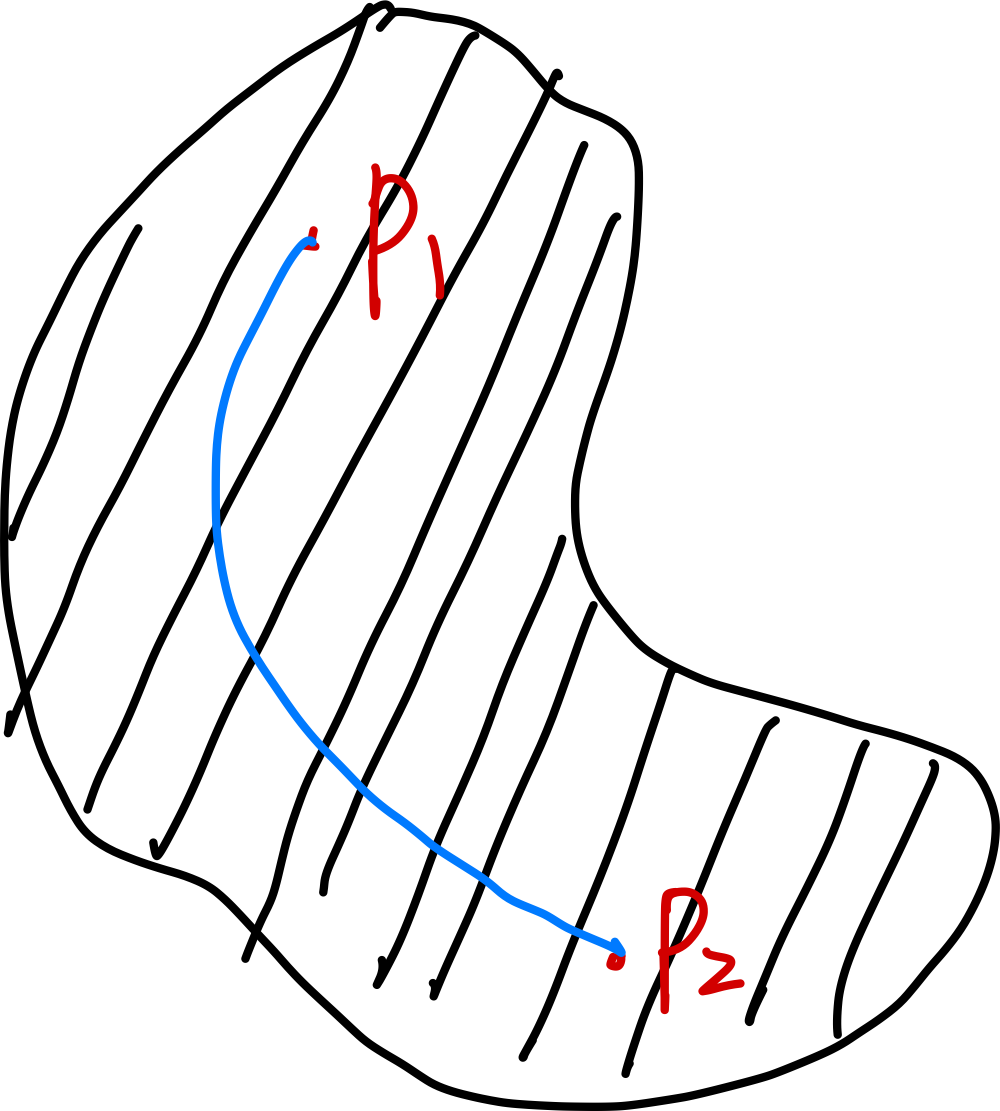
\includegraphics[scale=0.08]{"Chapter 09 images/pic1.png"}
            \end{minipage}
        }
        \subfigure[]
        {
             \begin{minipage}[b]{.3\linewidth}
                \centering
                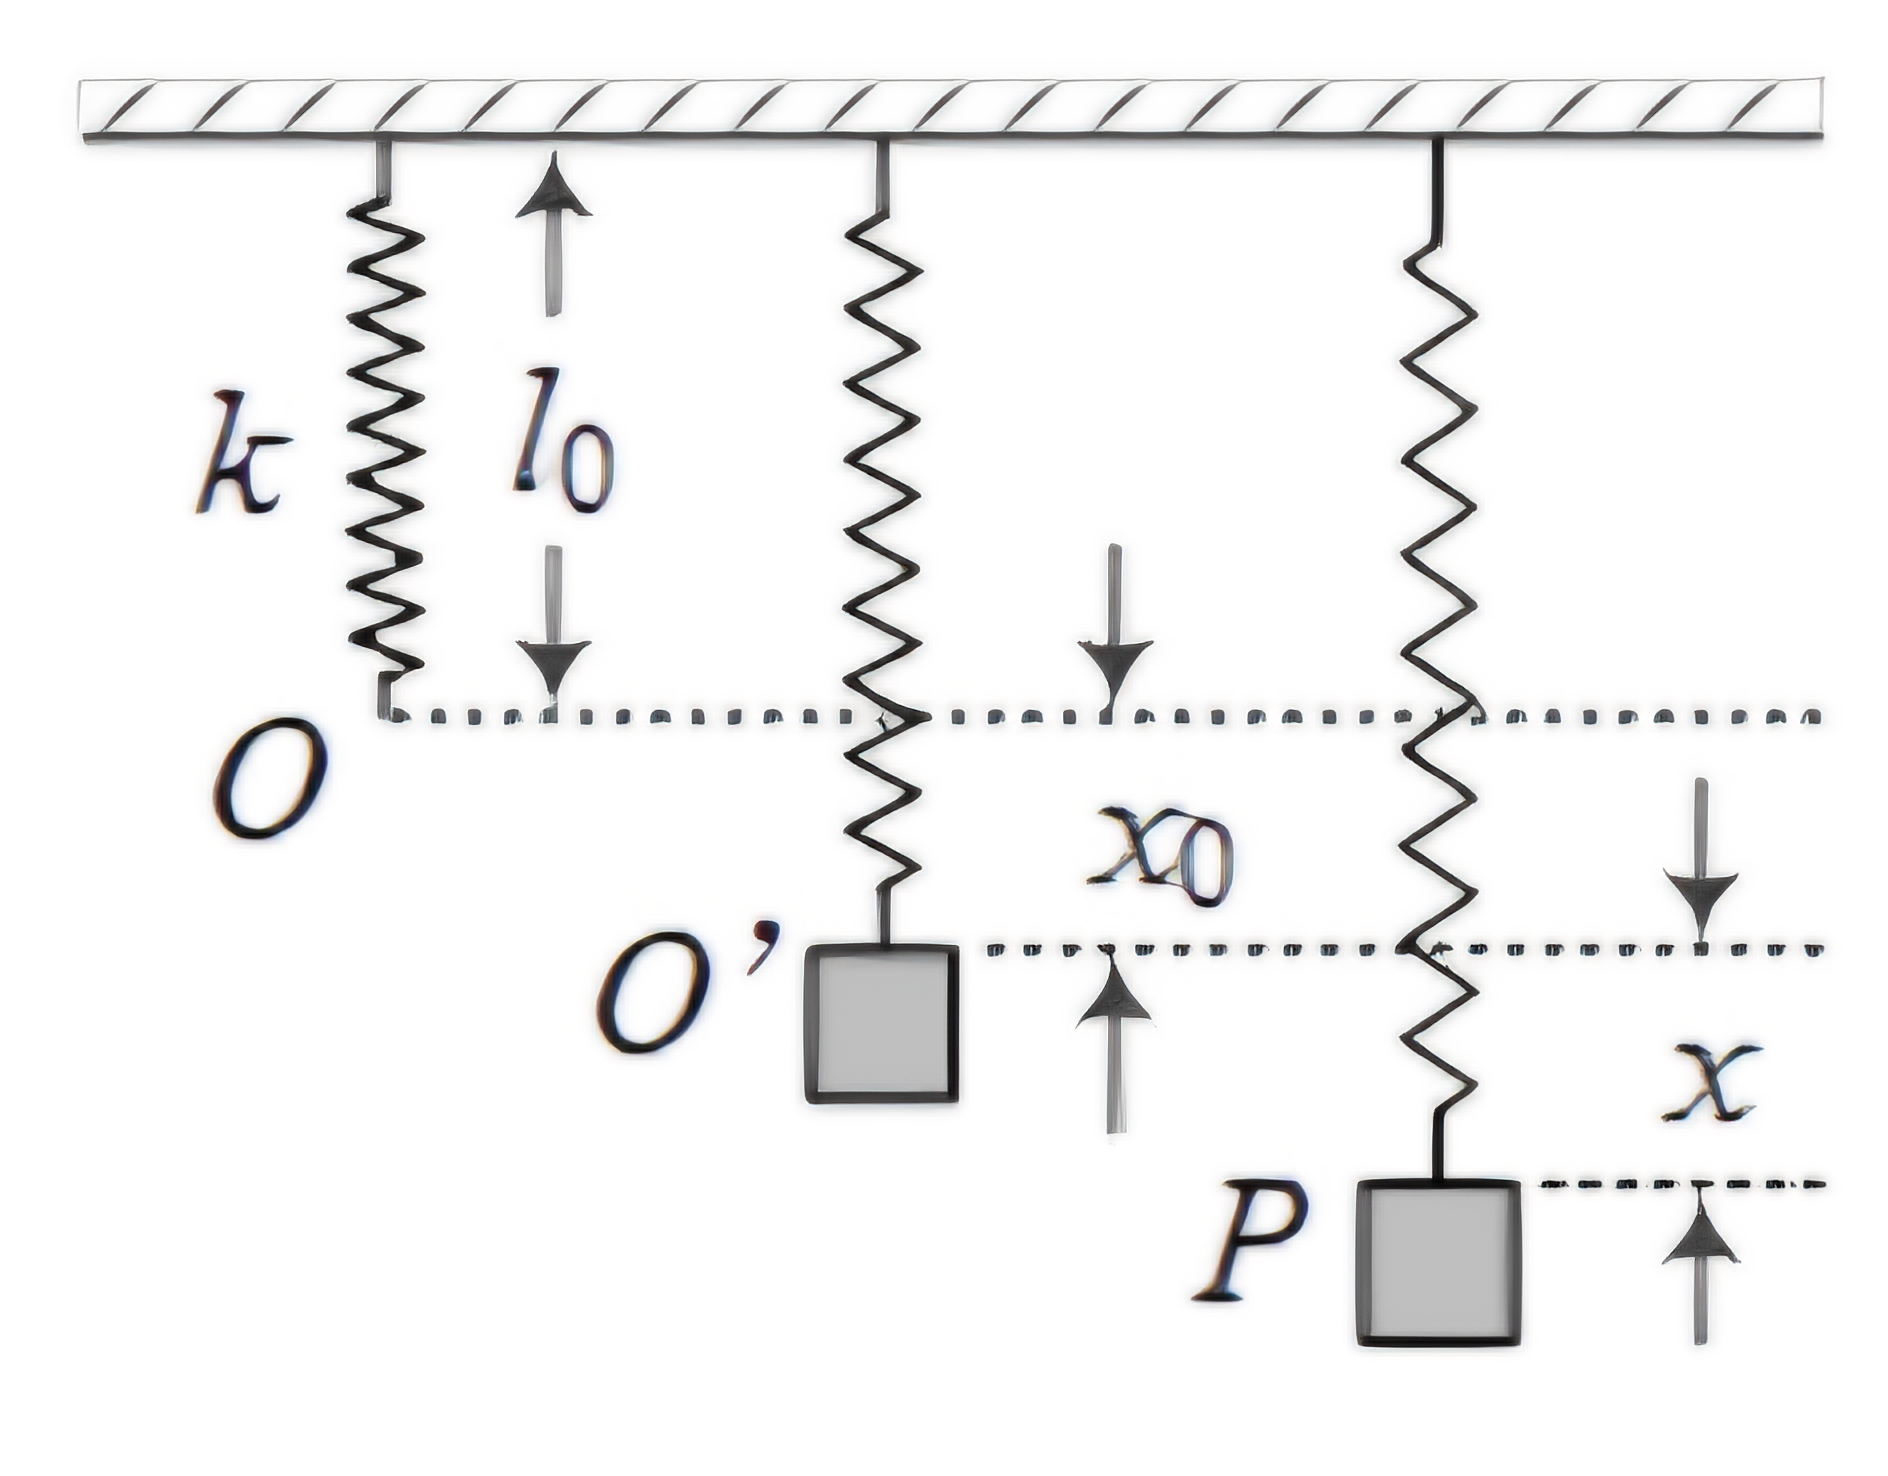
\includegraphics[scale=0.08]{"Chapter 09 images/pic2.jpg"}
            \end{minipage}
        }
    \end{figure}

    \begin{enumerate}
        \item 连通集:如上图(a);
        \item 非连通集:如上图(b)。
    \end{enumerate}

    \begin{enumerate}
        \item 开区域(也简称区域):连通的开集;
        \item 闭区域:开区域连同其边界一起构成的点集。
    \end{enumerate}

    如\(\left\{\left(x,y\right) \mid 1 < x^2+y^2 < 2\right\}\)
    为(开)区域;\(\left\{\left(x,y\right) \mid 1 \leq x^2+y^2 \leq 2\right\}\)
    为闭区域。

    \begin{enumerate}
        \item 有界集:对于集合\(E\),若\(\exists r > 0\),使\(E \subset U\left(0,r\right)\),
            则称\(E\)是有界的。(就是说能找到一个“圆”把集合\(E\)包裹起来)
        \item 无界集:若一个集合不是有界集,则称其为无界集。
    \end{enumerate}

    \begin{figure}[htbp]
        \centering
        \subfigure
        {
        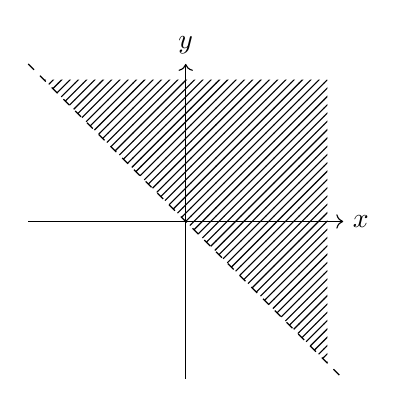
\begin{tikzpicture}
            \coordinate[label=right:$x$] (x) at (2,0);
            \coordinate[label=above:$y$] (y) at (0,2);
            \draw[->] (-2,0) -- (x);
            \draw[->] (0,-2) -- (y);
            \draw[dashed, domain=-2:2] plot(\x,{-\x});
            \fill[pattern=north east lines] (-1.8,1.8) -- (1.8,1.8) -- (1.8,-1.8);
        \end{tikzpicture}
        }
        \subfigure
        {
        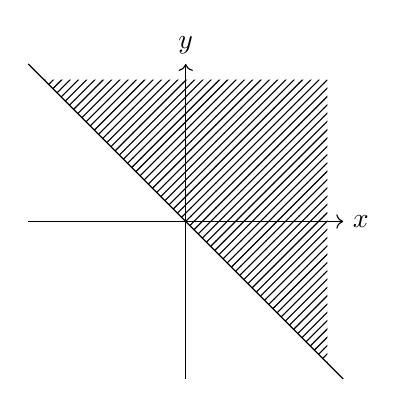
\begin{tikzpicture}
            \coordinate[label=right:$x$] (x) at (2,0);
            \coordinate[label=above:$y$] (y) at (0,2);
            \draw[->] (-2,0) -- (x);
            \draw[->] (0,-2) -- (y);
            \draw[domain=-2:2] plot(\x,{-\x});
            \fill[pattern=north east lines] (-1.8,1.8) -- (1.8,1.8) -- (1.8,-1.8);
        \end{tikzpicture}
        }
    \end{figure}

    例如,\(\left\{\left(x,y\right) \mid x + y > 0\right\}\)为无界开区域;
    \(\left\{\left(x,y\right) \mid x + y \geq 0\right\}\)为无界闭区域。

\subsection{多元函数的概念}

    \subsubsection{二元函数}

    设\(D\)是\(\mathbf{R}^2\)的一个非空子集,称映射\(f: D \rightarrow \mathbf{R}\)为定义在\(D\)上的二元函数,
    通常记为

    \begin{equation}
        z = f\left(x,y\right),\; \left(x,y\right) \in D
    \end{equation}

    或

    \begin{equation}
        z = f\left(P\right),\; P \in D
    \end{equation}

    \subsubsection{值域}

    上述定义中,与自变量\(x\)和y\(\)的一对值(即二元有序实数组)\(\left(x,y\right)\) 相对应的因变量\(z\)的值,
    也称为\(f\)在点\(\left(x,y\right)\)处的函数值,记作\(f\left(x,y\right)\),即\(z=f\left(x,y\right)\)
    函数值\(f\left(x,y\right)\)的全体所构成的集合为函数\(f\)的值域,记作\(f\left(D\right)\),即

    \begin{align}
        f\left(D\right) = \left\{z \mid z=f\left(x,y\right),\; \left(x,y\right) \in D\right\}
    \end{align}

    \subsubsection{推广}

    三元函数:\(u = f\left(x,y,z\right),\; \left(x,y,z\right) \in D\);

    \(n\)元函数:\(u = f\left(x_1,x_2,x_3,\ldots,x_n\right),\; \left(x_1,x_2,x_3,\ldots,x_n\right) \in D\)

    \subsubsection{自然定义域}

    使算式有意义的点的集合。
    
    例如\(z = \ln \left(x+y\right)\)的自然定义域为
    \(D = \left\{\left(x,y\right) \mid x + y > 0\right\}\)。\(z = \arcsin \left(x+y\right)\)
    的自然定义域为\(D = \left\{\left(x,y\right) \mid x^2 + y^2 \leq 1\right\}\)。

    \subsubsection{二元函数的图形}

    设函数\(z=f\left(x,y\right)\)的定义域为\(D\)。对于任意取定的点\(P(x,y) \in D\),
    对应的函数值为\(z=f\left(x,y\right)\)。这样,以\(x\)为横坐标,\(y\)为纵坐标和
    \(z=f\left(x,y\right)\)为竖坐标在空间就确定一点\(M\left(x,y,z\right)\)。
    当\(x,y\)遍取\(D\)上的一切点时,得到一个空间点集

    \begin{align}
        \left\{\left(x,y,z\right) \mid z=f\left(x,y\right),\; \left(x,y\right) \in D\right\}
    \end{align}
    
    这个点集称为二元函数\(z=f\left(x,y\right)\)的图形,通常我们也说二元函数的图形是一张曲面。

    例如,由空间解析几何知道,线性函数$z=ax+by+c$
    的图形是一张平面,而函数$z=x^2+y^2$的图形是旋转抛物面。

\subsection{多元函数的极限}

\subsubsection{二元函数的极限}

    如果在\(P\left(x,y\right) \rightarrow P_0\left(x_0,y_0\right)\)(即\(\left|PP_0\right| =
    \sqrt{\left(x-x_0\right)^2 + \left(y-y_0\right)^2} \rightarrow 0\))过程中,对应的函数值
    无限接近于一个确定的常数\(A\),那么就说\(A\)是函数\(f\left(x,y\right)\)当
    \(\left(x,y\right) \rightarrow \left(x_0,y_0\right)\)时的极限。

    \textbf{定义}:“\(\varepsilon - \delta\)”语言

    设二元函数 $f(P)=f(x, y)$ 的定义域为 $D$,$P_0\left(x_0, y_0\right)$
    是$D$的聚点。如果存在常数$A$,对于任意给定的正数$\varepsilon$,总存在正数$\delta$,
    使得当点$P(x, y) \in D \cap \ddot{U}\left(P_0, \delta\right)$ 时,都有

    \begin{equation}
        \left|f(P)-A\right|=\left|f(x, y)-A\right|<\varepsilon
    \end{equation}

    成立,那么就称常数\(A\)为函数\(f\left(x,y\right)\)当\(\left(x,y\right) \rightarrow \left(x_0,y_0\right)\)
    的极限,记作

    \begin{equation}
        \lim _{P \rightarrow P_0} f(P)=A \quad
    \end{equation}

    或

    \begin{equation}
        f(P) \rightarrow A\left(P \rightarrow P_0\right)
    \end{equation}

    \textbf{注意}:

    \begin{enumerate}
        \item \(P_0\)是\(D\)的聚点;
        \item 证明过程中,核心在于寻找\(\delta = \delta\left(\varepsilon\right)\)。
    \end{enumerate}

\end{document}
